\documentclass{article}

\usepackage[english]{babel}
\usepackage[utf8]{inputenc}
\usepackage{amsmath}
\usepackage{amsthm}
\usepackage{amssymb}
\usepackage{mathtools}
\usepackage{amsfonts}
\usepackage{subcaption}
\usepackage{graphicx}
\usepackage{wrapfig}
\usepackage{bbm}
\usepackage{dsfont}
\usepackage{listings}

% set up margin
\usepackage
[
  a4paper,
  left=3cm,
  right=3cm,
  top=3cm,
  bottom=3cm,
]
{geometry}

% set up header
\usepackage{fancyhdr}
\pagestyle{fancy}
\fancyhf{}
\lhead{6.438 Algorithms for Inference}
\chead{Problem Set 5}
\rhead{Hongzi Mao}
\cfoot{\thepage}
\rfoot{\footnotesize{\emph{Collaborated with: Hongzhou Ye, Zhiwei Ding}}}

% footer line
\renewcommand{\footrulewidth}{0.4pt}

% sans serif italic
\newcommand{\s}[1]{\textsf{\textit{#1}}}

% bold face sans serif
\newcommand{\bs}[1]{\textsf{\textbf{#1}}}

% set symbol
\usepackage[mathscr]{euscript}

% empty set
\let\emptyset\varnothing

% qed
\newcommand{\qeds}{\hfill\qedsymbol}

% math bold face
\newcommand{\bm}{\mathbf}

% argmax
\DeclareMathOperator*{\argmax}{argmax}
\DeclareMathOperator*{\argmin}{argmin}

% colorful reference
\usepackage{hyperref}
\usepackage{color}
\definecolor{darkred}{rgb}{0.7,0,0}
\definecolor{darkgreen}{rgb}{0,0.5,0}
\hypersetup{colorlinks=true,
        linkcolor=darkred,
        citecolor=darkgreen}
\urlstyle{same}

% independence symbol
\makeatletter
\newcommand*{\indep}{%
  \mathbin{%
    \mathpalette{\@indep}{}%
  }%
}
\newcommand*{\nindep}{%
  \mathbin{%                   % The final symbol is a binary math operator
    \mathpalette{\@indep}{\not}% \mathpalette helps for the adaptation
                               % of the symbol to the different math styles.
  }%
}
\newcommand*{\@indep}[2]{%
  \sbox0{$#1\perp\m@th$}%        box 0 contains \perp symbol
  \sbox2{$#1=$}%                 box 2 for the height of =
  \sbox4{$#1\vcenter{}$}%        box 4 for the height of the math axis
  \rlap{\copy0}%                 first \perp
  \dimen@=\dimexpr\ht2-\ht4-.2pt\relax
  \kern\dimen@
  {#2}
  \kern\dimen@
  \copy0 %                       second \perp
} 
\makeatother

%%%%%%%%%%%%%%%%%%%%%%%%%%%%%%%%%%%%%%%%%%%%%%%%%%%%%%%%%%%%%%%%%%%%%%%%
%%%%%%%%%%%%%%%%%%%%%%%%% Begin document here %%%%%%%%%%%%%%%%%%%%%%%%%%
%%%%%%%%%%%%%%%%%%%%%%%%%%%%%%%%%%%%%%%%%%%%%%%%%%%%%%%%%%%%%%%%%%%%%%%%
\begin{document}

\section*{Problem 5.1}
%
(a) We check local consistency by checking the marginals sum to 1 and the
edge marginals marginalize to node marginal. That is
%
\begin{align*}
	b_i(0) + b_i(1) = 0.5 + 0.5 = 1,
\end{align*}
%
for $\forall i \in \{1, 2, 3\}$; and
\begin{align*}
	b_{ij}(0,0) + b_{ij}(0,1) + b_{ij}(1,0) + b_{ij}(1,1) = 1,
\end{align*}
%
for $\forall i, j \in \{1, 2, 3\}, i \neq j$;
and\footnote{$b_i(1)$ checks out similarly for $\forall \{1,2,3\}$}
%
\begin{align*}
	b_{12}(0, 0) + b_{12}(0, 1) = 0.49 + 0.01 = 0.5 &= b_1(0),\\
	b_{12}(1, 0) + b_{12}(0, 0) = 0.01 + 0.49 = 0.5 &= b_2(0),\\
	b_{32}(0, 0) + b_{32}(0, 1) = 0.49 + 0.01 = 0.5 &= b_3(0),\\
	b_{32}(1, 0) + b_{32}(0, 0) = 0.01 + 0.49 = 0.5 &= b_2(0),\\
	b_{31}(0, 0) + b_{31}(0, 1) = 0.01 + 0.49 = 0.5 &= b_3(0),\\
	b_{31}(1, 0) + b_{31}(0, 0) = 0.49 + 0.01 = 0.5 &= b_1(0).\\
\end{align*} \qeds
%
\\

\noindent
(b) We prove this by contradiction. Suppose such distribution
$p_{\s{x}_1, \s{x}_2, \s{x}_3}(x_1, x_2, x_3)$ exists, then
\begin{align}
	&p_{\s{x}_1, \s{x}_2, \s{x}_3}(0, 0, 0) + p_{\s{x}_1, \s{x}_2, \s{x}_3}(0, 0, 1) = b_{12}(0, 0) = 0.49, \label{51b1}\\
	&p_{\s{x}_1, \s{x}_2, \s{x}_3}(0, 0, 0) + p_{\s{x}_1, \s{x}_2, \s{x}_3}(0, 1, 0) = b_{31}(0, 0) = 0.01, \label{51b2}\\
	&p_{\s{x}_1, \s{x}_2, \s{x}_3}(0, 0, 1) + p_{\s{x}_1, \s{x}_2, \s{x}_3}(1, 0, 1) = b_{32}(0, 1) = 0.01. \label{51b3}
\end{align}
%

Since we assume $p_{\s{x}_1, \s{x}_2, \s{x}_3}(\cdot)$ is a valid distribution, we have
\begin{align*}
	p_{\s{x}_1, \s{x}_2, \s{x}_3}(x_1, x_2, x_3) \geq 0,
\end{align*}
for $\forall (x_1, x_2, x_3) \in \{0, 1\}^3$.

Now, from Equation~\eqref{51b2}, we have
\begin{align*}
	p_{\s{x}_1, \s{x}_2, \s{x}_3}(0, 0, 0) \leq 0.01,
\end{align*}
from Equation~\eqref{51b3}, we have
\begin{align*}
	p_{\s{x}_1, \s{x}_2, \s{x}_3}(0, 0, 1) \leq 0.01.
\end{align*}
%

Thus, 
\begin{align*}
	p_{\s{x}_1, \s{x}_2, \s{x}_3}(0, 0, 0) + p_{\s{x}_1, \s{x}_2, \s{x}_3}(0, 0, 1) \leq 0.01 + 0.01 = 0.02,
\end{align*}
%
which contradicts with Equation~\eqref{51b1}, where 
$p_{\s{x}_1, \s{x}_2, \s{x}_3}(0, 0, 0) + p_{\s{x}_1, \s{x}_2, \s{x}_3}(0, 0, 1) = 0.49$.
\qeds
\\
\\
\\
\\
\\
\\
\\
\\
\\
\\

\pagebreak
%
%%%%%%%%%%%%%%%%%%%%%%%%%%%%%%%%%%%%%%%%%%%%%%%%%%%%%%%%%%%%%%%%%%%%%%%% 
\section*{Problem 5.2}
(a) With slight abuse of notations, we index the node with the coordinate
$(i, j)$ in the image. Figure~\ref{f:52a} sketches the undirected graphs.
%
\begin{figure}[h]
  \centering
  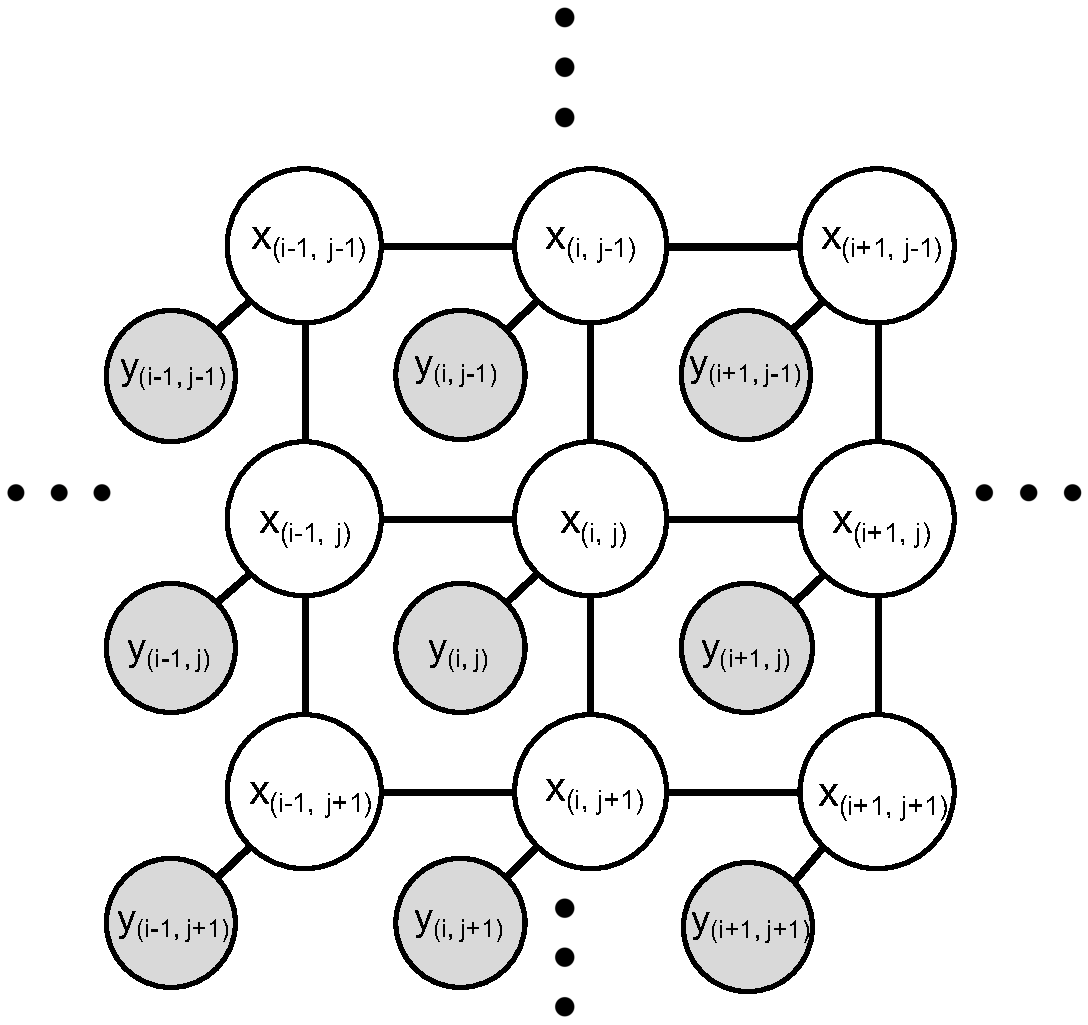
\includegraphics[width=0.4\columnwidth]{52a.pdf}
    \vspace{-0.1cm}
  \caption{Undirected graph of the 5.2 photography problem.}
  \label{f:52a}
\end{figure}
%

The potential function $\psi(x_i, y_i)$ is given by
\begin{align*}
	\psi(x_i, y_i) = p_{\s{y}_i|\s{x}_i}(y_i|x_i)
	= \frac{1}{(2\pi)^{3/2}(\det {\bf\Lambda}_{x_i})^{1/2}}
	\exp\left[-\frac{1}{2}(y_i-\mu_{x_i})^T\mathbf{\Lambda}^{-1}_{x_i}(y_i - \mu_{x_i})\right] + \epsilon.
\end{align*}
\\

\noindent
(b) For the labeled masks, we empirically compute
\begin{align*}
	&\mu_\alpha = \frac{1}{N_\alpha}\sum_{i=1}^{N_\alpha}y_i,\\
	&\mathbf{\Lambda}_{\alpha} = \frac{1}{N_\alpha}\sum_{i=1}^{N_\alpha}\left[(y_i - \mu_\alpha)(y_i - \mu_\alpha)^T\right],
\end{align*}
where $N_\alpha$ is the number of pixels in the labeled mask.
%

In the \texttt{flower} example, normalizing the pixel value
in the range $[0, 1]$ instead of $[0, 255]$, we have for the foreground
%
\begin{align*}
	\mu_1 = 
	\begin{bmatrix}
    0.7006 \\
    0.4504 \\
    0.0438
\end{bmatrix}, \;\;\,
	\mathbf{\Lambda}_1 =
\begin{bmatrix}
 0.0513 & 0.0598 & 0.0014 \\
 0.0598 & 0.8336 & 0.0023 \\
 0.0014 & 0.0023 & 0.0011
\end{bmatrix},
\end{align*}
and the background
\begin{align*}
	\mu_0 = 
	\begin{bmatrix}
    0.3249 \\
    0.3359 \\
    0.1549
\end{bmatrix}, \;\;\,
	\mathbf{\Lambda}_0 =
\begin{bmatrix}
0.0760 & 0.0709 & 0.0402 \\
0.0709 & 0.0672 & 0.0385 \\
0.0402 & 0.0385 & 0.0264
\end{bmatrix}.
\end{align*}

The code for this computation is attached in the bottom.
\\

\noindent
(c)
We denote the indices of the neighboring pixels of $j$ as $\partial j$. That is the observation $y_j$ is not a member of $\partial j$ and we consider the message from it separately. The update rule for the message passing is
\begin{align*}
	m_{j\to k}(x_k) &= \sum_{x_j} \psi_{jk}(x_j, x_k)\,\,m_{y_j\to x_j}(x_j) \prod_{l\in\partial{j}\backslash\{k\}}m_{l\to j}(x_j)\\
	&\propto \sum_{x_j} \big[0.9\times\mathds{1}_{x_j = x_k} + 0.1\times\mathds{1}_{x_j \neq x_k} \big] \times\\
	& \left\{\frac{1}{(2\pi)^{3/2}(\det {\bf\Lambda}_{x_j})^{1/2}} \exp\left[-\frac{1}{2}(y_j-\mu_{x_j})^T\mathbf{\Lambda}^{-1}_{x_j}(y_j - \mu_{x_j})\right] + \epsilon\right\}
	\times \prod_{l\in\partial{j}\backslash\{k\}}m_{l\to j}(x_j).
\end{align*}
%

To compute the marginal, the final belief update rule on $x_i$ is
\begin{align*}
	p_{\s{x}_i}(x_i) &\propto  m_{y_i\to x_i}(x_i) \prod_{j\in\partial{i}}m_{j\to i}(x_i)\\
	&\propto \left\{\frac{1}{(2\pi)^{3/2}(\det {\bf\Lambda}_{x_i})^{1/2}} \exp\left[-\frac{1}{2}(y_i-\mu_{x_i})^T\mathbf{\Lambda}^{-1}_{x_i}(y_i - \mu_{x_i})\right] + \epsilon\right\}
	\times \prod_{j\in\partial{i}}m_{j\to i}(x_i).
\end{align*}
\\

\noindent
(d) We visualize the pixel marginals in Figure~\ref{f:52d}.
%
The ``weak'' beliefs are the pixels with grey colors. That is, the underlining
marginals spreads the probability mass between foreground and background.
%
In early iterations (e.g., iteration 1 and 2), there are a few black-grey dots inside
the flower foreground regions. These pixels in the original graph looks a bit green-ish,
which leads to a large probability value in the observation-pixel edge Gaussian
distribution. Over time, the neighboring pixels will overcome this belief and ``absorb''
those grey dots by foreground belief in white.
%

The loopy BP first converges the clear values---red flowers in the foreground, with mean 
close to the empirical foreground mean, and the object clusters close each other; green 
grass in the background for similar reasons. There are an green ``island'' in the left
flower that is difficult to converge to the foreground. The reason is that it has a
significant size of green inside the flower red, which self-reinforce its background
position inside the foreground region.
%
\begin{figure*}[t]
\captionsetup[subfigure]{labelformat=empty}
\centering
%
\begin{subfigure}[t]{0.19\textwidth}
\centering

\includegraphics[width=\textwidth]{./images/marginals_iter_1.png}
\vspace{-0.6cm}
\caption{iteration=1}
\end{subfigure}
\begin{subfigure}[t]{0.19\textwidth}
\centering

\includegraphics[width=\textwidth]{./images/marginals_iter_2.png}
\vspace{-0.6cm}
\caption{iteration=2}
\end{subfigure}
\begin{subfigure}[t]{0.19\textwidth}
\centering

\includegraphics[width=\textwidth]{./images/marginals_iter_3.png}
\vspace{-0.6cm}
\caption{iteration=3}
\end{subfigure}
\begin{subfigure}[t]{0.19\textwidth}
\centering

\includegraphics[width=\textwidth]{./images/marginals_iter_4.png}
\vspace{-0.6cm}
\caption{iteration=4}
\end{subfigure}
\begin{subfigure}[t]{0.19\textwidth}
\centering

\includegraphics[width=\textwidth]{./images/marginals_iter_5.png}
\vspace{-0.6cm}
\caption{iteration=5}
\end{subfigure}
\begin{subfigure}[t]{0.19\textwidth}
\centering

\includegraphics[width=\textwidth]{./images/marginals_iter_6.png}
\vspace{-0.6cm}
\caption{iteration=6}
\end{subfigure}
\begin{subfigure}[t]{0.19\textwidth}
\centering

\includegraphics[width=\textwidth]{./images/marginals_iter_7.png}
\vspace{-0.6cm}
\caption{iteration=7}
\end{subfigure}
\begin{subfigure}[t]{0.19\textwidth}
\centering

\includegraphics[width=\textwidth]{./images/marginals_iter_8.png}
\vspace{-0.6cm}
\caption{iteration=8}
\end{subfigure}
\begin{subfigure}[t]{0.19\textwidth}
\centering

\includegraphics[width=\textwidth]{./images/marginals_iter_9.png}
\vspace{-0.6cm}
\caption{iteration=9}
\end{subfigure}
\begin{subfigure}[t]{0.19\textwidth}
\centering

\includegraphics[width=\textwidth]{./images/marginals_iter_10.png}
\vspace{-0.6cm}
\caption{iteration=10}
\end{subfigure}
\begin{subfigure}[t]{0.19\textwidth}
\centering

\includegraphics[width=\textwidth]{./images/marginals_iter_11.png}
\vspace{-0.6cm}
\caption{iteration=11}
\end{subfigure}
\begin{subfigure}[t]{0.19\textwidth}
\centering

\includegraphics[width=\textwidth]{./images/marginals_iter_12.png}
\vspace{-0.6cm}
\caption{iteration=12}
\end{subfigure}
\begin{subfigure}[t]{0.19\textwidth}
\centering

\includegraphics[width=\textwidth]{./images/marginals_iter_13.png}
\vspace{-0.6cm}
\caption{iteration=13}
\end{subfigure}
\begin{subfigure}[t]{0.19\textwidth}
\centering

\includegraphics[width=\textwidth]{./images/marginals_iter_14.png}
\vspace{-0.6cm}
\caption{iteration=14}
\end{subfigure}
\begin{subfigure}[t]{0.19\textwidth}
\centering

\includegraphics[width=\textwidth]{./images/marginals_iter_15.png}
\vspace{-0.6cm}
\caption{iteration=15}
\end{subfigure}
\begin{subfigure}[t]{0.19\textwidth}
\centering

\includegraphics[width=\textwidth]{./images/marginals_iter_16.png}
\vspace{-0.6cm}
\caption{iteration=16}
\end{subfigure}
\begin{subfigure}[t]{0.19\textwidth}
\centering

\includegraphics[width=\textwidth]{./images/marginals_iter_17.png}
\vspace{-0.6cm}
\caption{iteration=17}
\end{subfigure}
\begin{subfigure}[t]{0.19\textwidth}
\centering

\includegraphics[width=\textwidth]{./images/marginals_iter_18.png}
\vspace{-0.6cm}
\caption{iteration=18}
\end{subfigure}
\begin{subfigure}[t]{0.19\textwidth}
\centering

\includegraphics[width=\textwidth]{./images/marginals_iter_19.png}
\vspace{-0.6cm}
\caption{iteration=19}
\end{subfigure}
\begin{subfigure}[t]{0.19\textwidth}
\centering

\includegraphics[width=\textwidth]{./images/marginals_iter_20.png}
\vspace{-0.6cm}
\caption{iteration=20}
\end{subfigure}
\begin{subfigure}[t]{0.19\textwidth}
\centering

\includegraphics[width=\textwidth]{./images/marginals_iter_21.png}
\vspace{-0.6cm}
\caption{iteration=21}
\end{subfigure}
\begin{subfigure}[t]{0.19\textwidth}
\centering

\includegraphics[width=\textwidth]{./images/marginals_iter_22.png}
\vspace{-0.6cm}
\caption{iteration=22}
\end{subfigure}
\begin{subfigure}[t]{0.19\textwidth}
\centering

\includegraphics[width=\textwidth]{./images/marginals_iter_23.png}
\vspace{-0.6cm}
\caption{iteration=23}
\end{subfigure}
\begin{subfigure}[t]{0.19\textwidth}
\centering

\includegraphics[width=\textwidth]{./images/marginals_iter_24.png}
\vspace{-0.6cm}
\caption{iteration=24}
\end{subfigure}
\begin{subfigure}[t]{0.19\textwidth}
\centering

\includegraphics[width=\textwidth]{./images/marginals_iter_25.png}
\vspace{-0.6cm}
\caption{iteration=25}
\end{subfigure}
\begin{subfigure}[t]{0.19\textwidth}
\centering

\includegraphics[width=\textwidth]{./images/marginals_iter_26.png}
\vspace{-0.6cm}
\caption{iteration=26}
\end{subfigure}
\begin{subfigure}[t]{0.19\textwidth}
\centering

\includegraphics[width=\textwidth]{./images/marginals_iter_27.png}
\vspace{-0.6cm}
\caption{iteration=27}
\end{subfigure}
\begin{subfigure}[t]{0.19\textwidth}
\centering

\includegraphics[width=\textwidth]{./images/marginals_iter_28.png}
\vspace{-0.6cm}
\caption{iteration=28}
\end{subfigure}
\begin{subfigure}[t]{0.19\textwidth}
\centering

\includegraphics[width=\textwidth]{./images/marginals_iter_29.png}
\vspace{-0.6cm}
\caption{iteration=29}
\end{subfigure}
\begin{subfigure}[t]{0.19\textwidth}
\centering

\includegraphics[width=\textwidth]{./images/marginals_iter_30.png}
\vspace{-0.6cm}
\caption{iteration=30}
\end{subfigure}

%
\caption{Visualizing the expectation in pixel marginals. The foreground is indicated by white.}
\label{f:52d}
\end{figure*}

\pagebreak
The code for this problem is
\lstset{language=Python}
\lstset{frame=lines}
\lstset{caption={Using parallel sum product algorithm for separating
image foreground and background}}
\lstset{label={code:photography}}
\lstset{basicstyle=\footnotesize}
\begin{lstlisting}
import numpy as np
from scipy import misc
from bp import belief_propagation
from mean_var import compute_mean_var


def normalize_img(img):
    normalized_img = np.zeros(img.shape)
    for i in range(img.shape[0]):
        for j in range(img.shape[1]):
            for k in range(3):
                normalized_img[i, j, k] = float(img[i, j, k]) / 255.0
    return normalized_img


def visualize_marginals(img, marginals, file_name):
    array = np.zeros([img.shape[0], img.shape[1]])
    for (i, j) in marginals:
        array[i, j] = marginals[(i, j)][0]
    array = 1 - array  # revert black & white
    array *= 255
    misc.imsave(file_name, array)


def main():
    image_file = './images/flower.bmp'
    foreground_file = './images/foreground.bmp'
    background_file = './images/background.bmp'

    image = misc.imread(image_file, flatten= 0)
    image = normalize_img(image)  # between [0, 1]
    foreground = misc.imread(foreground_file, flatten= 0)
    background = misc.imread(background_file, flatten= 0)

    mean_foreground, var_foreground = \
        compute_mean_var(image, foreground)

    mean_background, var_background = \
        compute_mean_var(image, background)

    mean_foreground = mean_foreground.reshape(-1, 1)
    mean_background = mean_background.reshape(-1, 1)

    det_foreground = np.linalg.det(var_foreground)
    det_background = np.linalg.det(var_background)

    inv_foreground = np.linalg.inv(var_foreground)
    inv_background = np.linalg.inv(var_background)

    eps = 0.01

    # neighbor pixel edge potentials
    psi_neighbors = {}
    psi_neighbors[(0, 0)] = 0.9
    psi_neighbors[(1, 1)] = 0.9
    psi_neighbors[(0, 1)] = 0.1
    psi_neighbors[(1, 0)] = 0.1

    # fill in the potential functions
    node_potential = {}
    edge_potential = {}

    for i in range(image.shape[0]):
        for j in range(image.shape[1]):
            # node potential is influenced by the observation
            img_vec = image[i,j].reshape(-1, 1)
            node = {}
            node[1] = 1 / ((2 * np.pi) ** (3/2) * det_foreground ** (1/2)) * \
                np.exp(-0.5 * ((img_vec - mean_foreground).T.dot(inv_foreground)).dot(
                (img_vec - mean_foreground))) + eps
            node[0] = 1 / ((2 * np.pi) ** (3/2) * det_background ** (1/2)) * \
                np.exp(-0.5 * ((img_vec - mean_background).T.dot(inv_background)).dot(
                (img_vec - mean_background))) + eps
            node_potential[(i, j)] = node
            # edge potential among the pixels
            if i - 1 >= 0:
                if ((i - 1, j), (i, j)) not in edge_potential:
                    edge_potential[((i, j), (i - 1, j))] = psi_neighbors
            if i + 1 < image.shape[0]:
                if ((i + 1, j), (i, j)) not in edge_potential:
                    edge_potential[((i, j), (i + 1, j))] = psi_neighbors
            if j - 1 >= 0:
                if ((i, j - 1), (i, j)) not in edge_potential:
                    edge_potential[((i, j), (i, j - 1))] = psi_neighbors
            if j + 1 < image.shape[1]:
                if ((i, j + 1), (i, j)) not in edge_potential:
                    edge_potential[((i, j), (i, j + 1))] = psi_neighbors

    # get marginal at every step
    d = 0
    for marginals in belief_propagation(node_potential, edge_potential, 30):
        d += 1
        visualize_marginals(image, marginals,
            './images/marginals_iter_' + str(d) + '.png')
        print('Step', d)


if __name__ == '__main__':
    main()
\end{lstlisting}

The library code \texttt{bp.py} (inherited from pset 3) is
\lstset{language=Python}
\lstset{frame=lines}
\lstset{caption={bp.py}}
\lstset{label={code:bp}}
\lstset{basicstyle=\footnotesize}
\begin{lstlisting}
import numpy as np


def ep(edge_potential, i, j, var_i, var_j):
    if (i, j) in edge_potential:
        return edge_potential[(i, j)][var_i, var_j]
    elif (j, i) in edge_potential:
        return edge_potential[(j, i)][var_j, var_i]
    else:
        return None


def get_msg(i, j, node_potential, edge_potential, messages, neighbors, normalize=True):
    # get msg_{i->j}(var)
    distant_msg = {0: 1, 1: 1}
    for k in neighbors[i]:
        if k != j:
            distant_msg[0] *= messages[(k, i)][0]
            distant_msg[1] *= messages[(k, i)][1]

    msg = {}
    msg[0] = node_potential[i][0] * ep(edge_potential, i, j, 0, 0) * distant_msg[0] \
           + node_potential[i][1] * ep(edge_potential, i, j, 1, 0) * distant_msg[1]
    msg[1] = node_potential[i][0] * ep(edge_potential, i, j, 0, 1) * distant_msg[0] \
           + node_potential[i][1] * ep(edge_potential, i, j, 1, 1) * distant_msg[1]

    if normalize:
        s = msg[0] + msg[1]
        msg[0] /= s
        msg[1] /= s

    return msg


def normalize_marginals(marginals):
    for node in marginals:
        p_sum = marginals[node][0] + marginals[node][1]
        marginals[node][0] /= p_sum
        marginals[node][1] /= p_sum


def belief_propagation(node_potential, edge_potential, diameter=np.inf):
    '''
    node_potential: {i -> node_potential}
    edge_potential: {(i, j) -> edge_potential}
    output: {i -> marginal}
    '''
    
    # find neighbor nodes for each node
    neighbors = {}
    for i in node_potential:
        neighbors[i] = set()
    for (i, j) in edge_potential:
        neighbors[i].add(j)
        neighbors[j].add(i)

    # initialize random message
    messages = {}
    init_msg = {0: 1, 1: 1}
    for (i, j) in edge_potential:
        messages[(i, j)] = init_msg
        messages[(j, i)] = init_msg

    diam = min(diameter, len(node_potential))

    # tree diameter <= total number of nodes
    for _ in range(diam):
        new_messages = {}
        for i in node_potential:
            for j in neighbors[i]:
                msg = get_msg(
                    i, j,
                    node_potential,
                    edge_potential,
                    messages,
                    neighbors)
                new_messages[(i, j)] = msg
        assert len(new_messages) == len(messages)
        messages = new_messages

        # compute marginals
        marginals = {}
        for i in node_potential:
            marginals[i] = {}
            msg = {0: 1, 1: 1}
            for j in neighbors[i]:
                msg[0] *= messages[(j, i)][0]
                msg[1] *= messages[(j, i)][1]
            marginals[i][0] = node_potential[i][0] * msg[0]
            marginals[i][1] = node_potential[i][1] * msg[1]

        # normalize marginals
        normalize_marginals(marginals)

        yield marginals

\end{lstlisting}

The axillary code for computing empirical mean and covariance is 
\lstset{language=Python}
\lstset{frame=lines}
\lstset{caption={mean\_var.py}}
\lstset{label={code:bp}}
\lstset{basicstyle=\footnotesize}
\begin{lstlisting}
import numpy as np
from scipy import misc


def compute_mean_var(image, ground):
    num_pixels = 0
    mean = np.zeros(3)
    sum_val = np.zeros(3)

    assert image.shape[0] == ground.shape[0]
    assert image.shape[1] == ground.shape[1]

    for i in range(image.shape[0]):
        for j in range(image.shape[1]):
            if ground[i, j] > 0:
                sum_val += image[i, j]
                num_pixels += 1

    if num_pixels > 0:
        mean = sum_val / num_pixels

    var = np.zeros([3, 3])
    sum_val = np.zeros([3, 3])

    for i in range(image.shape[0]):
        for j in range(image.shape[1]):
            if ground[i, j] > 0:
                val = (image[i, j] - mean).reshape(-1, 1)
                sum_val += val.dot(val.T)

    if num_pixels > 0:
        var = sum_val / num_pixels

    return mean, var

\end{lstlisting}
\pagebreak

%%%%%%%%%%%%%%%%%%%%%%%%%%%%%%%%%%%%%%%%%%%%%%%%%%%%%%%%%%%%%%%%%%%%%%%% 
\section*{Problem 5.3}
(a)
Since $p_{\bm{x}}(\mathbf{x}) = \mathscr{N}(\mathbf{x} | \mu, J^{-1})$, we have
\begin{align*}
	b_1^{t+1}(x_1) &= K' \exp\left\{\int b_2^{t}(x_2)
	\log\big[p_{\bm{x}}(\mathbf{x})\big]dx_2\right\} \\
	&= K' \exp\left\{\int b_2^{t}(x_2)
	\left[\log\left(\frac{1}{(2\pi)|J^{-1}|^{-\frac{1}{2}}}\right) - 
	\frac{1}{2}(\bm{x}-\mu)^T J (\bm{x}-\mu)\right]dx_2\right\}\\
	& = K''\exp\left\{-\frac{1}{2}\int b^t_2(x_2)
	\begin{bmatrix}
		x_1 - \mu_1 & x_2 - \mu_2 \\
	\end{bmatrix}
	\begin{bmatrix}
		J_{11} & J_{12} \\
		J_{21} & J_{22}
	\end{bmatrix}
	\begin{bmatrix}
		x_1 - \mu_1 \\
		x_2 - \mu_2
	\end{bmatrix}
	dx_2
\right\}\\
&\text{(note we absorb the constants in $K''$)}\\
&= K''\exp\bigg\{-\frac{1}{2}\bigg[J_{11}(x_1-\mu_1)^2 \int
b_2^t(x_2)dx_2 \\
&\;\;\;\;\;\;\;\;\;\;\;\;\;\;\;\;\;\;\;\;\;\;\;\;\;\;\;+
2J_{12}(x_1-\mu_1)\int b^t_2(x_2)(x_2-\mu_2)dx_2\\
&\;\;\;\;\;\;\;\;\;\;\;\;\;\;\;\;\;\;\;\;\;\;\;\;\;\;\;+
J_{22}\int b^t_2(x_2)(x_2-\mu_2)^2dx_2 \bigg]\bigg\}.
\end{align*}
%

Notice that $b_1^{t+1}(x_1)$ is a Gaussian density in $x_1$, regardless
of the distribution of $b_2^t(x_2)$ (since it is integrated out; and the Gaussian form will be more clear in Equation~\eqref{eq:53a1}).
%
To determine the normalization constant $K'$, we let
\begin{align*}
	x_1' &= x_1 - \mu_1 \\
	A &= J_{11}\int b_2^t(x_2)dx_2 \\
	B &= 2J_{12}\int b^t_2(x_2)(x_2-\mu_2)dx_2\\
	C & = J_{22}\int b^t_2(x_2)(x_2-\mu_2)^2dx_2,
\end{align*}
then
\begin{align}
	b_1^{t+1}(x_1) &= K''\exp\Big[-\frac{1}{2} \left(A x_1'^2 + B x_1' + C\right)\Big] \label{eq:53a1}.
\end{align}
%

By completing the square,
\begin{align*}
	b_1^{t+1}(x_1) &= K''\exp\Big[-\frac{1}{2}
	\frac{(x' - B/2A)^2 + C/A - B^2 / 4A^2}{1/A}\Big].
\end{align*}
%

Thus,
\begin{align}
	K'' = \frac{1}{\sqrt{2\pi/A}}\exp\left(\frac{C-B^2/4A}{2}\right),
\end{align}
%

and
\begin{align}
	K' = \frac{1}{\sqrt{2\pi/A}}\exp\left[\frac{C-B^2/4A}{2} -
	\log\left(\frac{1}{(2\pi)|J^{-1}|^{-\frac{1}{2}}}\right)
	\int b_2^{t}(x_2)dx_2\right].
\end{align}
%

Similarly, the expression for the $b_2^{t+1}(x_2)$ update is analogous
to~\eqref{eq:53a1} with factor $b_1^t$ switched in to the expression. 
\\

\noindent
(b)

\pagebreak

%%%%%%%%%%%%%%%%%%%%%%%%%%%%%%%%%%%%%%%%%%%%%%%%%%%%%%%%%%%%%%%%%%%%%%%% 
\section*{Problem 5.5}
(a) The computation trees corresponding to the first 4 iterations
are shown in Figure~\ref{f:55a}.
%
\begin{figure}[h]
  \centering
	\begin{subfigure}[t]{0.15\textwidth}
	\centering
	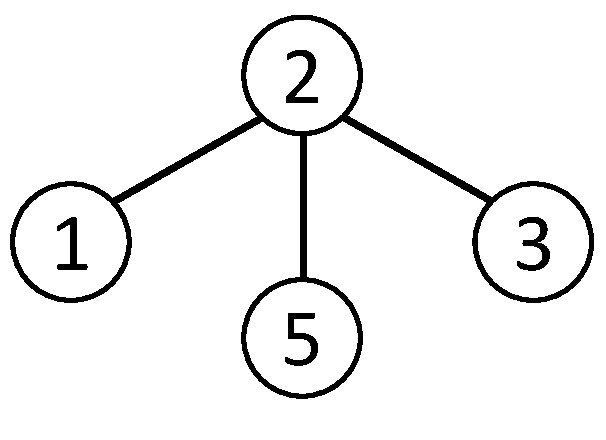
\includegraphics[width=\textwidth]{55a1.pdf}
	\vspace{-0.6cm}
	\caption{iteration=1.}
	\end{subfigure}
	%
		\begin{subfigure}[t]{0.23\textwidth}
	\centering
	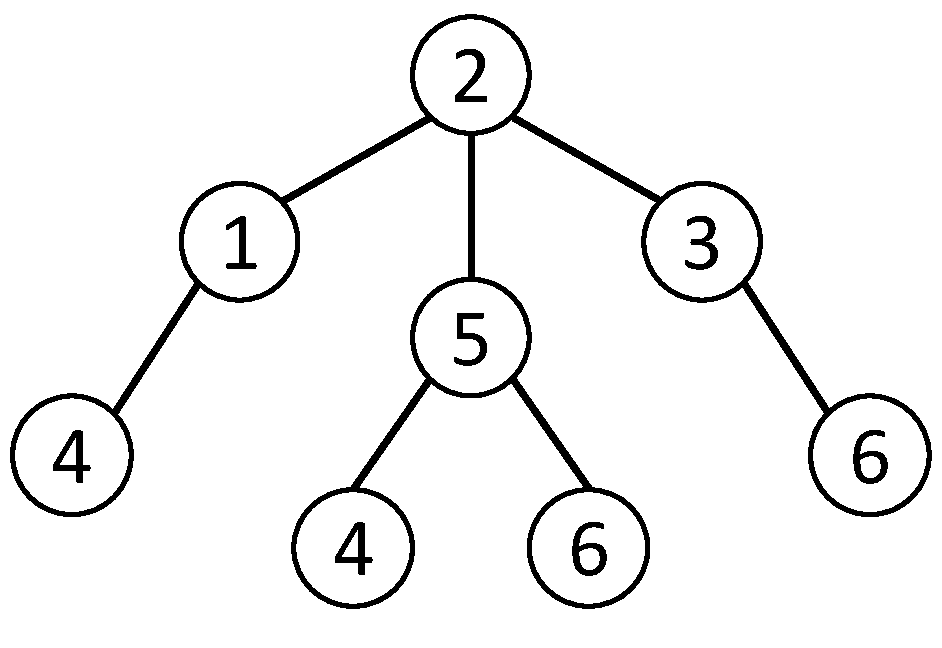
\includegraphics[width=\textwidth]{55a2.pdf}
	\vspace{-0.6cm}
	\caption{iteration=2.}
	\end{subfigure}
	%
		\begin{subfigure}[t]{0.23\textwidth}
	\centering
	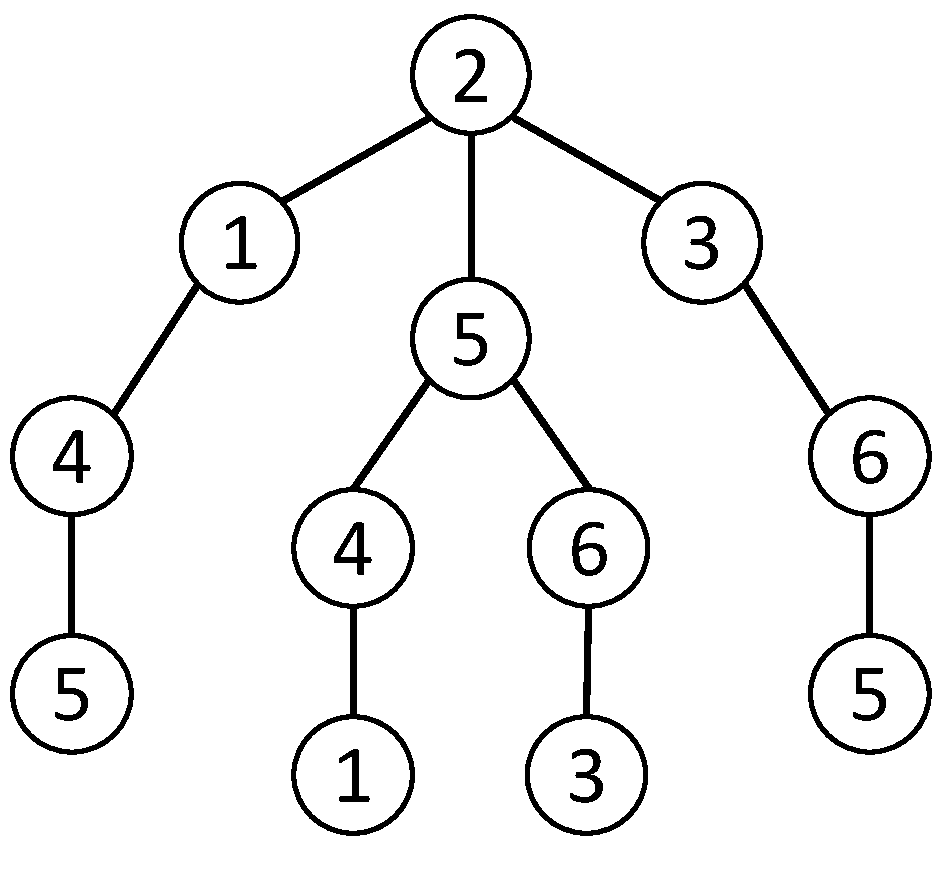
\includegraphics[width=\textwidth]{55a3.pdf}
	\vspace{-0.6cm}
	\caption{iteration=3.}
	\end{subfigure}
	%
		\begin{subfigure}[t]{0.29\textwidth}
	\centering
	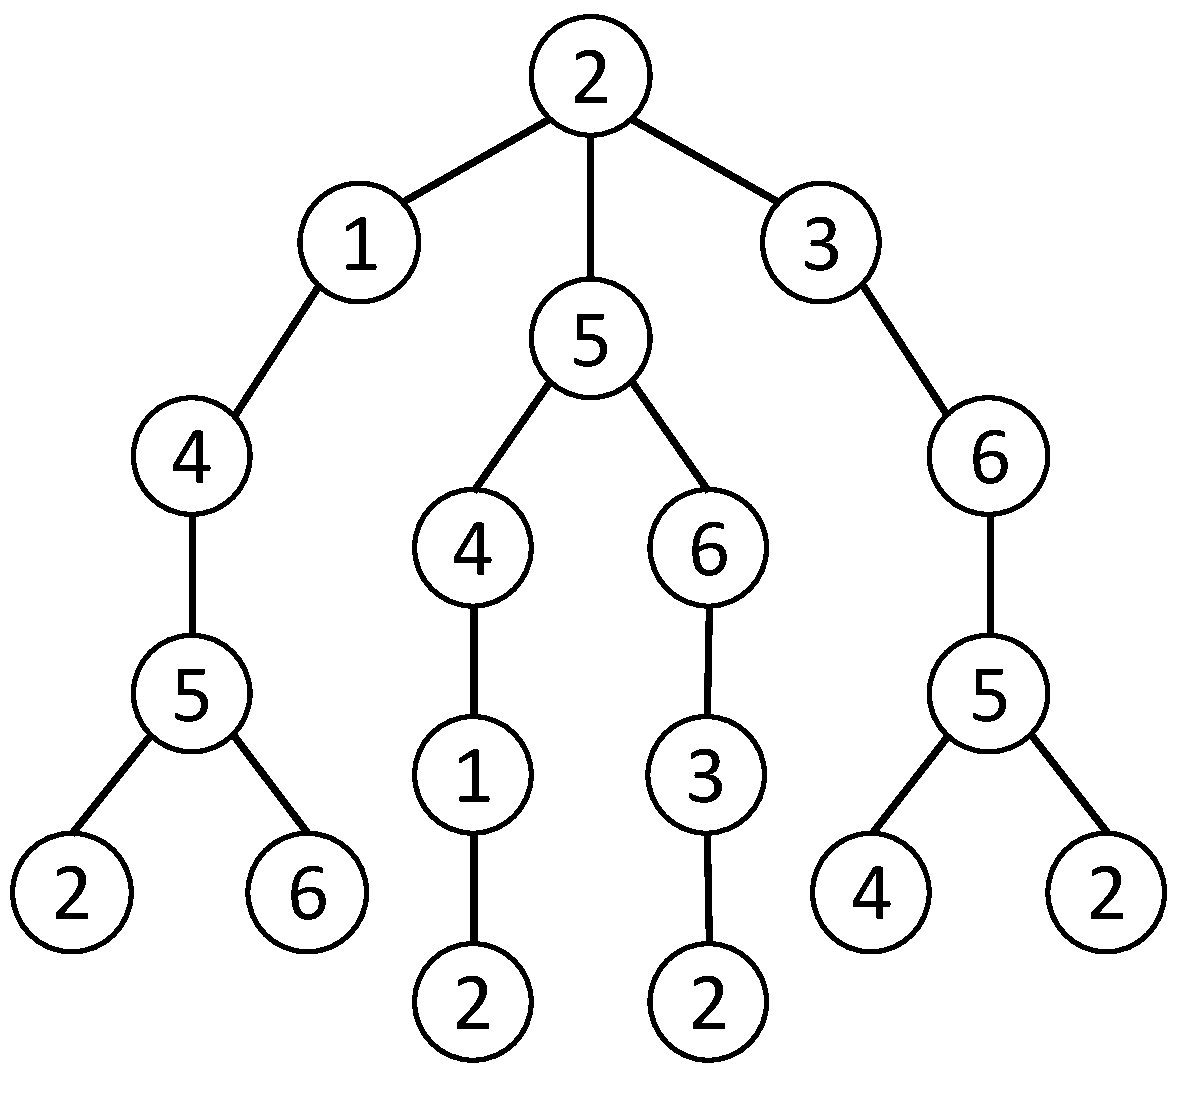
\includegraphics[width=\textwidth]{55a4.pdf}
	\vspace{-0.6cm}
	\caption{iteration=4.}
	\end{subfigure}
  \caption{Computation trees corresponding to the first 4
  iterations of loopy belief propagation.}
  \label{f:55a}
\end{figure}
%
\\

\noindent
(b) 
With the joint distribution, we can assign the node potential to $\s{x}_2$
and $\s{x}_5$ to be $\psi_2(x_2)$ and $\psi_2(x_5)$; constant 1 to all other nodes;
and edge potential $\mathds{1}_{x_i = x_j}$ to all edges $(i, j) \in \mathscr{E}$.
%
\\

\noindent
\textbf{Iteration 1.} Notice that for the message from $\s{x}_1$ and $\s{x}_3$,
%
\begin{align*}
	m^{t=1}_{1\to2}(x_2) &= \sum_{x_1}\mathds{1}_{x_1 = x_2} = 1,\\
	m^{t=1}_{3\to2}(x_2) &= \sum_{x_3}\mathds{1}_{x_3 = x_2} = 1.
\end{align*}
%
For the message from $\s{x}_5$,
%
\begin{align*}
	m^{t=1}_{5\to2}(x_2) &=
	\sum_{x_5}\psi_5(x_5)\mathds{1}_{x_5 = x_2} = \psi_5(x_2).
\end{align*}
%
Thus,
%
\begin{align*}
	p^{t=1}_{\s{x}_2}(x_2) \propto \psi_2(x_2)\psi_5(x_2).
\end{align*}
%
Specifically,
%
\begin{align}
	p^{t=1}_{\s{x}_2}(x_2=0) \propto \psi_2(0)\psi_5(0) = (1 - \gamma)\gamma,\\
	p^{t=1}_{\s{x}_2}(x_2=1) \propto \psi_2(1)\psi_5(1) = \gamma(1 - \gamma).
\end{align}
%
Hence, 
\begin{align}
	p^{t=1}_{\s{x}_2}(x_2=0) = p^{t=1}_{\s{x}_2}(x_2=1) = 0.5.
\end{align}

\noindent
\textbf{Iteration 2.} Notice that the message from $\s{x}_4$ to $\s{x}_1$ is
%
\begin{align*}
	m^{t=1}_{4\to1}(x_1) &= \sum_{x_4}\mathds{1}_{x_4 = x_1} = 1,
\end{align*}
%
and the same message applies to all leaves in iteration 2, $m^{t=1}_{4\to5}(x_5)$,
$m^{t=1}_{6\to5}(x_5)$ and $m^{t=1}_{6\to3}(x_3)$.
%
Thus, they do not influence the message passing to $\s{x}_2$ at iteration 2.
%
Therefore,
%
\begin{align}
	p^{t=2}_{\s{x}_2}(x_2=0) = p^{t=2}_{\s{x}_2}(x_2=1) = 0.5.
\end{align}

\noindent
\textbf{Iteration 3.} Notice that the messages from $\s{x}_5$ to $\s{x}_4$ and
$\s{x}_5$ to $\s{x}_6$ are
%
\begin{align*}
	m^{t=1}_{5\to4}(x_4) &= \sum_{x_5}\psi_5(x_5)\mathds{1}_{x_5 = x_4} = \psi_5(x_4),\\
	m^{t=1}_{5\to6}(x_6) &= \sum_{x_5}\psi_5(x_5)\mathds{1}_{x_5 = x_6} = \psi_5(x_6).
\end{align*}
%
Similar as before, the messages from from $\s{x}_1$ to $\s{x}_4$ and $\s{x}_3$ to $\s{x}_6$ are 1.
%
Since the message from leaves $\s{x}_5$ carries over all the way to $\s{x}_2$, we have
%
\begin{align}
	p^{t=3}_{\s{x}_2}(x_2=0) \propto \psi_5^3(0)\psi_2(0) = \gamma^3(1 - \gamma),\\
	p^{t=3}_{\s{x}_2}(x_2=1) \propto \psi_5^3(1)\psi_2(1) = (1 - \gamma)^3\gamma.
\end{align}
%
After normalization,
\begin{align}
	p^{t=3}_{\s{x}_2}(x_2=0) = 
		\frac{\gamma^2}{\gamma^2+ (1 - \gamma)^2},\\
	p^{t=3}_{\s{x}_2}(x_2=1) =
		\frac{(1 - \gamma)^2}{{\gamma^2 + (1 - \gamma)^2}}.
\end{align}

\noindent
\textbf{Iteration 4.} Notice that the message from $\s{x}_2$ to $\s{x}_5$ is
\begin{align*}
	m^{t=1}_{2\to5}(x_5) &= \sum_{x_2}\psi_2(x_2)\mathds{1}_{x_2 = x_5} = \psi_2(x_5).
\end{align*}
%
and the similar message applies to $m^{t=1}_{2\to1}(x_1)$,
$m^{t=1}_{2\to3}(x_3)$ and $m^{t=1}_{2\to5}(x_5)$.
%
Similar as before, the messages from from $\s{x}_6$ to $\s{x}_5$
and $\s{x}_4$ to $\s{x}_5$ are 1.
%
Since the messages carries over, e.g.,
\begin{align*}
	m^{t=2}_{5\to4}(x_4) &= \sum_{x_5}\psi_5(x_5)\mathds{1}_{x_5 = x_4}\psi_2(x_5)
	= \psi_5(x_4)\psi_2(x_4),
\end{align*}
%
we have
\begin{align}
	p^{t=4}_{\s{x}_2}(x_2=0) \propto \psi_5^3(0)\psi_2(0)^5 = \gamma^3(1 - \gamma)^5,\\
	p^{t=4}_{\s{x}_2}(x_2=1) \propto \psi_5^3(1)\psi_2(1)^5 = (1 - \gamma)^3\gamma^5.
\end{align}
%
After normalization,
\begin{align}
	p^{t=4}_{\s{x}_2}(x_2=0) = 
		\frac{(1 - \gamma)^2}{(1 - \gamma)^2 + \gamma^2},\\
	p^{t=4}_{\s{x}_2}(x_2=1) =
		\frac{\gamma^2}{{(1 - \gamma)^2 + \gamma^2}}.
\end{align}
\\

\noindent
(c) From the joint distribution, we directly have
\begin{align*}
	p_{\s{x}_1,\s{x}_2,\s{x}_3,\s{x}_4,\s{x}_5,\s{x}_6}(0,0,0,0,0,0) \propto
	\psi_2(0)\psi_5(0) = (1-\gamma)\gamma,\\
	p_{\s{x}_1,\s{x}_2,\s{x}_3,\s{x}_4,\s{x}_5,\s{x}_6}(1,1,1,1,1,1) \propto
	\psi_2(1)\psi_5(1) = \gamma(1-\gamma),
\end{align*}
and all other assignments of $\s{x}_i$ have probability 0 because of the edge constraints.
%

Thus, we have
\begin{align}
	p_{\s{x}_i}(0) = p_{\s{x}_i}(1) = 0.5,
\end{align}
for all $i\in\{1,2,3,4,5,6\}$.
%

Now focus on node $\s{x}_1$, to achieve this marginal, we have
\begin{align*}
	&p_{\s{x}_1}(0) = m_{2\to 1}(0) \times m_{4\to 1}(0)
				   = \beta \times m_{4\to 1}(0),\\
	&p_{\s{x}_1}(1) = m_{2\to 1}(1) \times m_{4\to 1}(1)
				   = (1-\beta) \times m_{4\to 1}(1).
\end{align*}
% 
Since $p_{\s{x}_1}(0) = p_{\s{x}_1}(1),$ we have
\begin{align}
	m_{4\to 1}(0) = 1- \beta, \label{5c1} \\
	m_{4\to 1}(1) = \beta \label{5c2}.
\end{align}
%
Similarly, we have
\begin{align}
	m_{6\to 3}(0) = 1- \alpha, \label{5c3} \\
	m_{6\to 3}(1) = \alpha. \label{5c4}
\end{align}
%
Now, we know the node potential on $\s{x}_1$, $\s{x}_4$, $\s{x}_3$ and
$\s{x}_6$ pertains constants. Thus,
\begin{align}
	m_{1\to 4}(0) = m_{2\to 1}(0) = \beta,\;\;\,
	m_{1\to 4}(1) = m_{2\to 1}(1) = 1 - \beta,\\
	m_{3\to 6}(0) = m_{2\to 3}(0) = \alpha,\;\;\,
	m_{3\to 6}(1) = m_{2\to 3}(1) = 1 - \alpha.
\end{align}
%
Using the similar argument for $\s{x}_4$
and $\s{x}_6$, we have
\begin{align}
	m_{4\to 5}(0) = m_{1\to 4}(0) = \beta,\;\;\,
	m_{4\to 5}(1) = m_{1\to 4}(1) = 1 - \beta,\\
	m_{6\to 5}(0) = m_{3\to 6}(0) = \alpha,\;\;\,
	m_{6\to 5}(1) = m_{3\to 6}(1) = 1 - \alpha.	
\end{align}
%
Now we consider the marginal on $\s{x}_5$, we have
\begin{align*}
	&p_{\s{x}_5}(0) = \psi_5(0) \times m_{4\to 5}(0) \times
					  m_{6\to 5}(0) \times m_{2\to 5}(0)
				   = \alpha\beta\gamma\, m_{2\to 5}(0),\\
	&p_{\s{x}_5}(1) = \psi_5(1) \times m_{4\to 5}(1) \times
					  m_{6\to 5}(1) \times m_{2\to 5}(1)
				   = (1-\alpha)(1-\beta)(1-\gamma)\, m_{2\to 5}(1).
\end{align*}
Therefore, let $m_{2\to5}(0) = m$, $m_{2\to5}(1) = 1 - m$,
\begin{align}
	\alpha\,\beta\,\gamma\,m = (1-\alpha)(1-\beta)(1-\gamma)(1-m). \label{55cc}
\end{align}
%
Notice that at this point, whatever $\alpha, \beta, m$ we choose, the message
passing equations will automatically satisfy the marginal constraint on $\s{x}_1$\footnote{As we will see at the end, the constraint is symmetrically  $(1-\alpha)(1-\beta)(1-\gamma)(1-m) = \alpha\,\beta\,\gamma\,m$.}, we get to choose $\alpha, \beta, m$ to let~\eqref{55cc} hold. The possible choices are
%
\begin{align}
	\alpha = 0.5, \beta = 1-\gamma;	
\end{align}
%
or
%
\begin{align}
	\alpha = 1-\gamma, \beta = 0.5;	
\end{align}
%
or
%
\begin{align}
	\alpha = 0.5, \beta = 0.5.
\end{align}
%
The corresponding $m$ corresponding to the above three choices are $0.5, 0.5, 1-\gamma$.
%

Similar to the argument about nodes $\s{x}_1, \s{x}_3$ do not carry variable node 
potentials, using
equations~\eqref{5c1}~\eqref{5c2}~\eqref{5c3}~\eqref{5c4}, we have the messages
\begin{align}
	m_{1\to 2}(0) = m_{4\to 1}(0) = 1 - \beta,\;\;\,
	m_{1\to 2}(1) = m_{4\to 1}(1) = \beta,\\
	m_{3\to 2}(0) = m_{6\to 3}(0) = 1 - \alpha,\;\;\,
	m_{3\to 2}(1) = m_{6\to 3}(1) = \alpha.
\end{align}
%
Similar to the argument about the marginal constraint on $\s{x}_2$, we have
%
\begin{align}
	(1-\alpha)(1-\beta)(1-\gamma)m_{5\to2}(0) = \alpha\,\beta\,\gamma\,m_{5\to2}(1),
\end{align}
%
Since $m_{5\to2}(0) + m_{5\to2}(1) = 1$, we have
%
\begin{align}
	m_{5\to2}(0) = \frac{\alpha\,\beta\,\gamma}{\alpha\,\beta\,\gamma +
	(1-\alpha)(1-\beta)(1-\gamma)},\\
	m_{5\to2}(1) = \frac{(1-\alpha)(1-\beta)(1-\gamma)
	}{\alpha\,\beta\,\gamma +
	(1-\alpha)(1-\beta)(1-\gamma)}.
\end{align}

\end{document}